\SubProblem
{تولید کدهای متعامد}
{
% OSVF %
\lr{\textbf{Orthogonal Variable Spreading Factor}}
یا
\lr{OSVF}
که با آن می‌توان یک درخت کد ایجاد کرد. این درخت یک درخت باینری با
\lr{K}
لایه است که هر راس آن نمایان‌گر یک کد برای ایجاد کانال است.

\begin{figure}[H]
    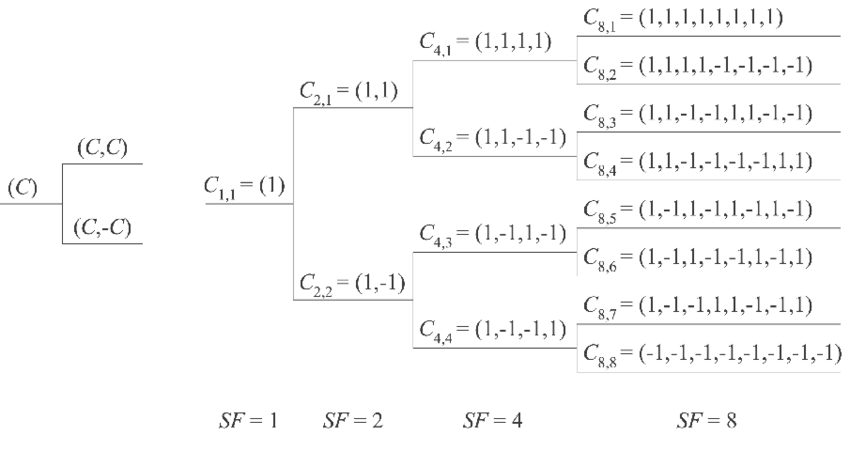
\includegraphics[width=15cm]{Images/OSVF.png}
    \centering
    \caption{\lr{OSVF Tree}}
\end{figure}

هر گره دو فرزند به صورت
\lr{(C, C)}
و
\lr{(C, C')}
دارد و کدهای تولید شده در هر طبقه از درخت بر هم عمود هستند.


% PN Seq %
\newpage
\lr{\textbf{Pseudo-Noise(PN) Sequence}}
توسط مولد نویز شبه تصادفی تولید می‌شود.
این مولد یک
\lr{Binary Linear Feedback Shift Register}
است که از مدارات
\lr{XOR}
و
\lr{Shift Register}
تشکیل شده است.

\begin{figure}[H]
    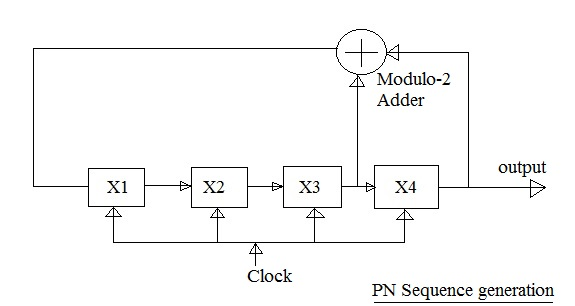
\includegraphics[width=10cm]{Images/PN.jpg}
    \centering
    \caption{\lr{PN Generator}}
\end{figure}


\begin{figure}[H]
    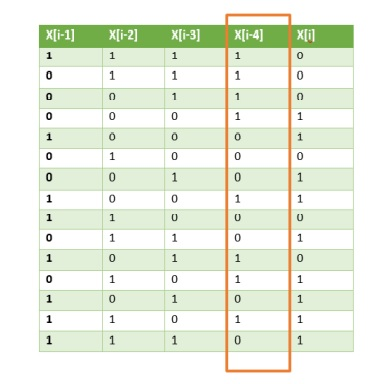
\includegraphics[width=10cm]{Images/PN_Table.jpg}
    \centering
    \caption{\lr{PN Table}}
\end{figure}

روش تولید رشته در جدول بالا نشان داده شده است خروجی مطلوب ما مقدار
\lr{X[i-4]}
است.
همانطور که در جدول زیر پیداست پس از به دست آوردن کد مورد نظر نیاز است تا صفر و یک‌ها را به سطوح ولتاژ تبدیل کنیم. از این رو به جای هر 0 مقدار 1 و به جای هر 1 مقدار -1 را قرار می‌دهیم.

\begin{equation*}
\begin{aligned}
    sequence = [-1,-1,-1,-1,1,1,1,-1,1,1,-1,-1,1,-1,1]
\end{aligned}
\end{equation*}

یکی از خواص این رشته تولید شده خاصیت
\lr{Cyclic Shift Property}
است. به این معنا که ضرب داخلی نرمالیزه شده شیفت یافته‌ها رشته به طور چرخشی، مقدار
\lr{$\frac{-1}{N}$}
را دارند.
اگر مقدار
\lr{N}
به سمت بی‌نهایت میل پیدا کند حاصل به سمت صفر میل خواهد کرد که حاکی از تعامد است.
در این روش رابطه زیر باید برقرار باشد.

\begin{equation*}
\begin{aligned}
    N = 2^n - 1
\end{aligned}
\end{equation*}


% Walsh %
\newpage
\lr{\textbf{Walsh matrix}}
یک ماتریس مربع خاص در ابعاد
\lr{$2^n$}
است.
درایه‌های این ماتریس اعداد مثبت یک یا منفی یک هستند.
در این ماتریس ردیف‌ها و ستون‌ها متعامد هستند.
هر ردیف این ماتریس مربوط به یک تابع
\lr{Walsh}
است.
این ماتریس به صورت بازگشتی محاسبه می‌شود که روابط آن به صورت زیر است.

\begin{equation*}
\begin{aligned}
    H(2^1) =
    \begin{bmatrix}
        1 & 1\\
        1 & -1
    \end{bmatrix}
\end{aligned}
\end{equation*}

\begin{equation*}
\begin{aligned}
    H(2^k) =
    \begin{bmatrix}
        H(2^{k-1}) & H(2^{k-1})\\
        H(2^{k-1}) & -H(2^{k-1})
    \end{bmatrix}
\end{aligned}
\end{equation*}

\begin{figure}[H]
    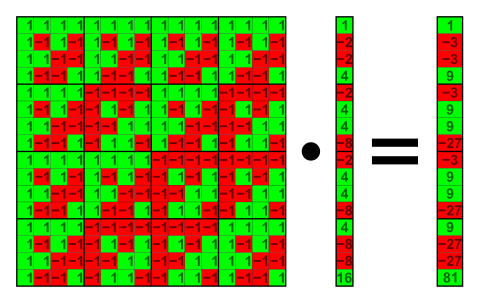
\includegraphics[width=15cm]{Images/Walsh.png}
    \centering
    \caption{\lr{Walsh Matrix}}
\end{figure}
}